\begin{titlepage}
\thispagestyle{empty}
\begin{tikzpicture}[remember picture,overlay]
  % 整页星图背景（左侧已烘焙深色渐隐，保证文字对比度）
  \node[inner sep=0pt] at (current page.center)
    {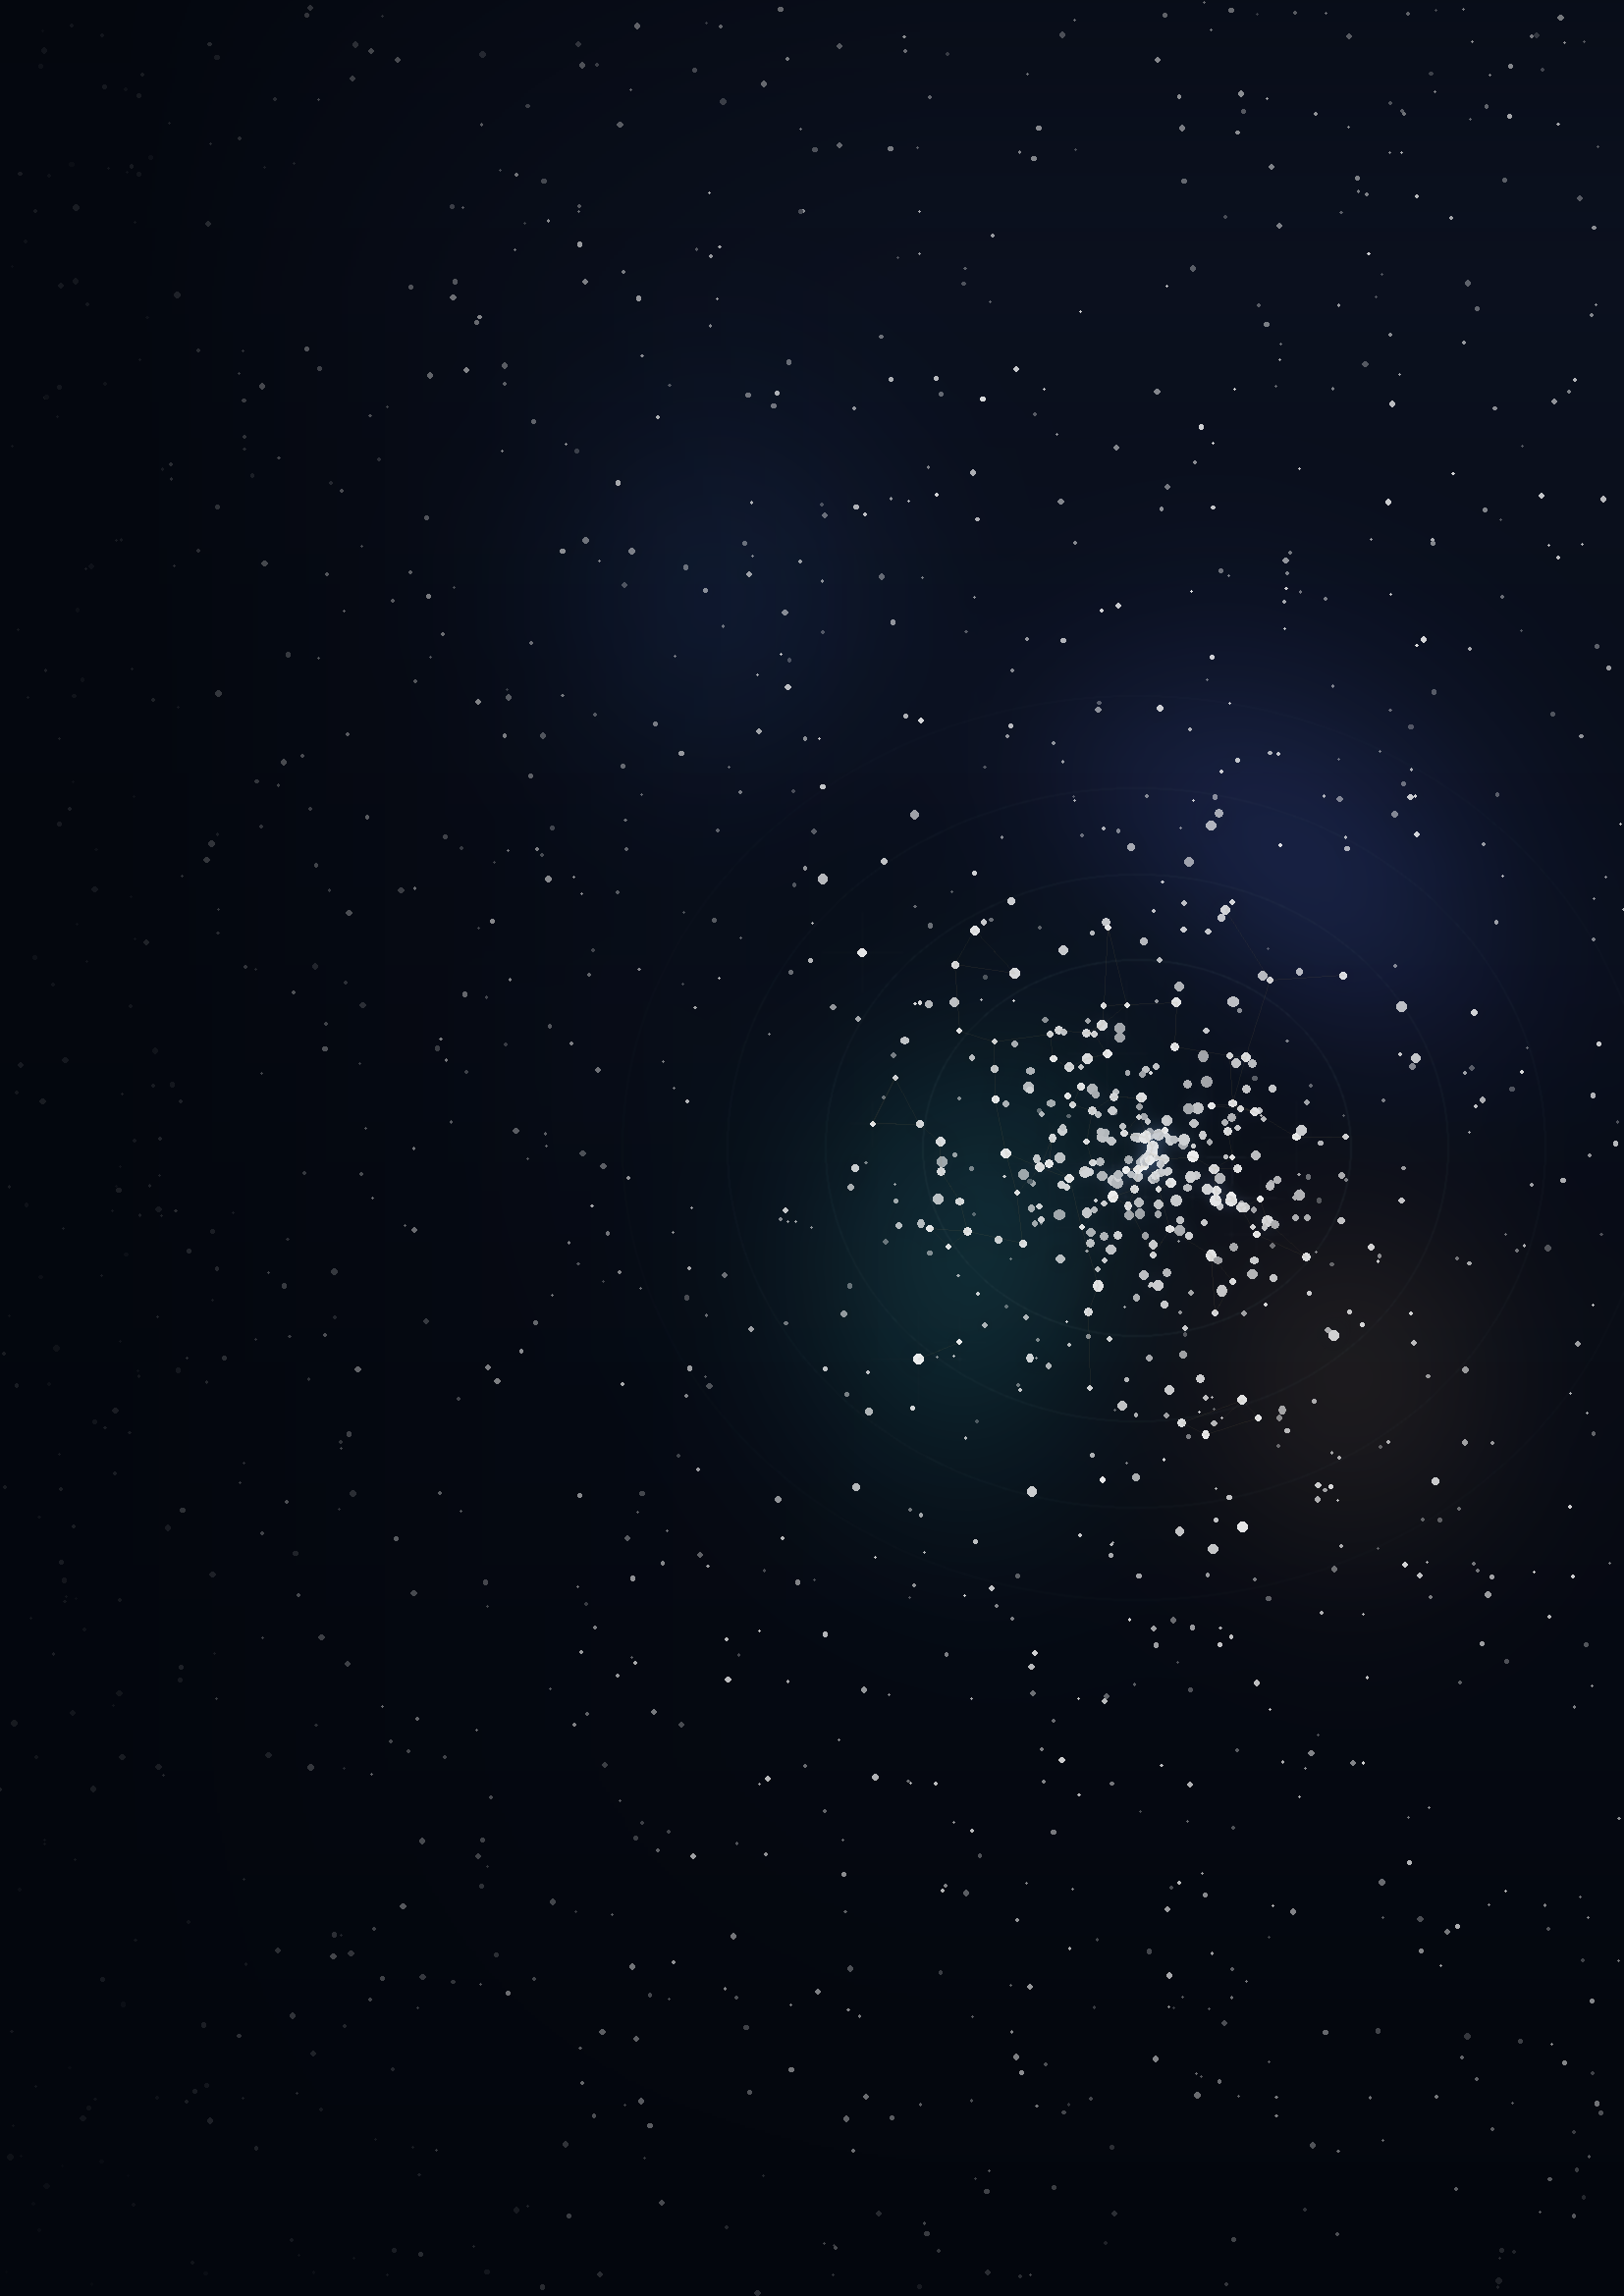
\includegraphics[width=\paperwidth,height=\paperheight]{figures/cover-bg.png}};

  % 顶部赛事标识
  \node[anchor=north west,text width=15.5cm,align=left]
    at ([xshift=2.15cm,yshift=-1.85cm]current page.north west)
    {\color{white!90}\heiti\small 2026 第九届“传智杯”全国大学生数智创新与 AI 应用大赛\\
     \color{white!62}\footnotesize AI WEB 网页开发挑战赛 · 赛道 10037 · RAG 知识问答系统};

  % 主标题
  \node[anchor=west,text width=14cm,align=left]
    at ([xshift=2.15cm,yshift=1.72cm]current page.west)
    {\color{white}\heiti\fontsize{47}{55}\selectfont StellarLit};
  \node[anchor=west,text width=14cm,align=left]
    at ([xshift=2.15cm,yshift=0.55cm]current page.west)
    {\color{white!95}\heiti\fontsize{25}{32}\selectfont 论文星图};
  \node[anchor=west,text width=14cm,align=left]
    at ([xshift=2.15cm,yshift=-0.55cm]current page.west)
    {\color{gold}\heiti\fontsize{16}{22}\selectfont 技术文档};

  \draw[gold,line width=0.8pt] ([xshift=2.15cm,yshift=-1.35cm]current page.west) -- ++(4.2cm,0);

  \node[anchor=west,text width=11.6cm,align=left]
    at ([xshift=2.15cm,yshift=-2.35cm]current page.west)
    {\color{white!92}\large 把一篇论文，长成一片星空。\\[4pt]
     \color{white!74}\normalsize 可核验的关系图谱 · 可追问的文献工作台};

  % 底部信息
  \node[anchor=south west,text width=15.6cm,align=left]
    at ([xshift=2.15cm,yshift=1.45cm]current page.south west)
    {\color{white!94}\heiti\normalsize 西安交通大学 · 白白 BAB · 研究生组\\[3pt]
     \color{white!72}\small 指导教师：白秀秀\quad|\quad 队员：薛志恒（队长）、张子桦、陈林涛};
  \node[anchor=south east]
    at ([xshift=-2.15cm,yshift=1.45cm]current page.south east)
    {\color{white!68}\small v1.0 · 2026 年 11 月};
\end{tikzpicture}
\end{titlepage}
